\documentclass[12pt]{jarticle}
\usepackage{graphicx}
\textwidth=16cm
\oddsidemargin=0cm

\newcommand \Br [1] {\left( #1 \right)}

\renewcommand  \[  {\begin{eqnarray}}
\renewcommand  \]  {\end{eqnarray}}

\begin{document}


\title{工学基礎実験実習 やさしいC言語\\最終レポート}%2%
\date{出題日: 2019年7月9日 \\
      提出日: \today \\
      締切日: 2019年7月23日 \\} 
\author{氏名:重近大智\\学生番号:09501527}
\maketitle

\section{はじめに}
本レポートでは,ニュートン法を用いて,与えられた4つの課題を解く.まず,ニュートン法の式を反復するC言語プログラムの作成方針を示し,.

\section{ニュートン法の原理}
\label{sec:bas}

方程式$f(x)=0$の解は,関数$f(x)=0$を満たす$x$のことである.
図\ref{fig:newton-kaishaku}では,曲線$y=f(x)$と$x$軸が交わっており,この交点の$x$座標が$x_k$である.

点$(x_k,f(x_k))$における曲線$y=f(x)$の接線の方程式$y=f(x_k)+(x-x_k)\cdot f\prime(x_k)$は,$f(x)$の導関数であることが分かる.
この接線と$x$軸の交点($x_{k+1}$)は次の式で表される\cite{clo05,mathwld}.これがニュートン法の基本の式である.
\[
x_{k+1}=x_k-\frac{f(x_k)}{f'(x_k)}
\label{eq:newton}
\]
図\ref{fig:newton-kaishaku}の場合,$x_{k+1}$が$x_k$よりも求める解$x$に近い.このため,
適当な初期値$x_0$を与え,式(\ref{eq:newton})によって数列$(x_k)$を
定義すると,この数列は$k\rightarrow\infty$で求める$x$に近付き,収束することが
期待される.

\begin{figure}[t]
  \center
  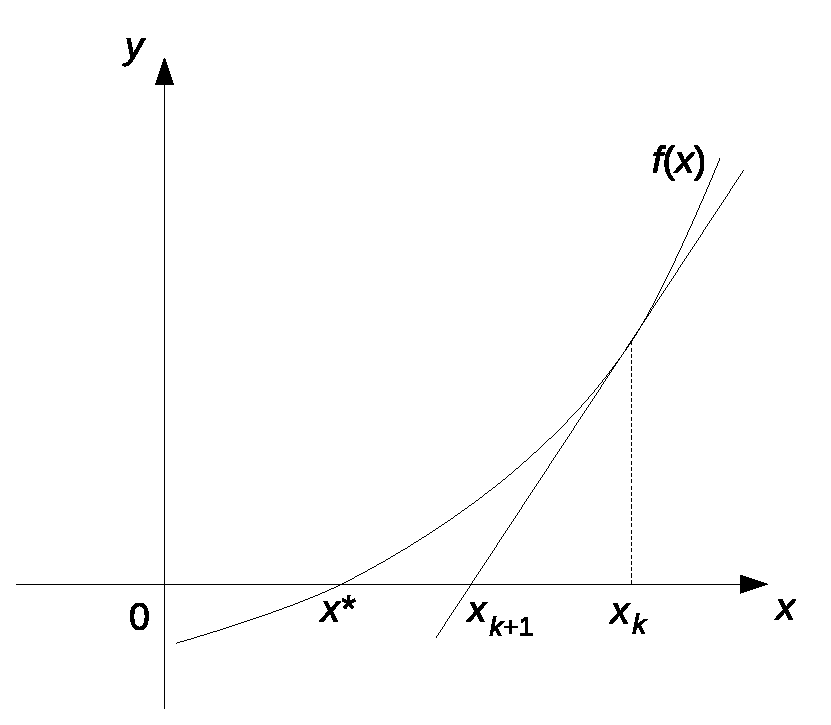
\includegraphics[scale=.6]{newton-kaishaku.eps}
  \caption{ニュートン法の幾何学的解釈}
  \label{fig:newton-kaishaku}
\end{figure}

収束性の議論を厳密にするために,真の解$x$との誤差$r_k$を次のように定
義する.
\[
\label{eq:deferr}
r_k := x_k - x
\]

%付け加えてください.f(x_k)について説明すること.%

\section{実験}
\label{sec:exp}
課題で与えられた関数に関する図,また用いたC言語プログラムのソースはレポートの最後にまとめて表示する.
\subsection{課題1}
課題1で与えられた方程式は次の3つである.
\begin{equation}
\sin e^x = 0
\label{eq:1-am}
\end{equation}
\begin{equation}
x^3-3x-2 = 0
\label{eq:1-bm}
\end{equation}
\begin{equation}
x^3-x^2-x+1 = 0
\label{eq:1-cm}
\end{equation}
まず,1つ目の方程式(式\ref{eq:1-am})について考える.方程式の解は,$f(x)=\sin\pi=0$
と考えると,$e^x=\pi$となるから,$x=\log\pi$が解である.
導関数は$f\prime(x)=e^x\cos e^x$であるから,ニュートン法の反復式は次のようになる.
\[
\label{eq:1-a}
x_{k+1}=x_k- \frac{\sin e^{x_k}}{e^{x_k}\cos e^{x_k}}
\]
初期値$x_0$を$1$とし,C言語プログラムで式\ref{eq:1-a}の反復計算を行った.結果を表\ref{tab:1-a}に示す.


\begin{table}[t]
 \caption{1つ目の方程式に関する反復回数と求められた解の近似値}
 \label{tab:1-a}
 \center
\begin{tabular}{|c|c|}
\hline
反復回数 &求められた解の近似値 \\
\hline
1  & 1.1657479108 \\
2  & 1.1449182997 \\
3  & 1.1447299036 \\
4  & 1.1447298858 \\
5  & 1.1447298858 \\
\hline
 \end{tabular}
\end{table}


次に,2つ目の方程式(式\ref{eq:1-bm})について考える.方程式の解は,$f(x)=x^3-3x-2=0$
と考えると,$x=-1$が解の1つとなる.

導関数は$f\prime(x)=3x^2-3$であるから,ニュートン法の反復式は次のようになる.
\[
\label{eq:1-b}
x_{k+1}=x_k- \frac{x_k^3-3x_k-2}{3x_k^2-3}
\]
初期値$x_0$を$-8$とし,C言語プログラムで式\ref{eq:1-b}の反復計算を行った.結果を表\ref{tab:1-b}に示す.ただし,収束するまで回数を要したため,最後の5回のみを表示する.


\begin{table}[t]
 \caption{2つ目の方程式に関する反復回数と求められた解の近似値}
 \label{tab:1-b}
 \center
\begin{tabular}{|c|c|}
\hline
反復回数 &求められた解の近似値 \\
\hline
28  & -1.0000000712 \\
29  & -1.0000000349 \\
30  & -1.0000000189 \\
31  & -1.0000000111 \\
32  & -1.0000000045 \\
\hline
 \end{tabular}
\end{table}

次に,3つ目の方程式(式\ref{eq:1-cm})について考える.方程式の解は,$f(x)=x^3-x^2-x+1=0$
と考えると,$x=1$が解の1つとなる.

導関数は$f\prime(x)=3x^2-2x-1$であるから,ニュートン法の反復式は次のようになる.
\[
\label{eq:1-c}
x_{k+1}=x_k- \frac{x_k^3-x_k^2-x_k+1}{3x_k^2-2x_k-1}
\]
初期値$x_0$を$6$とし,C言語プログラムで式\ref{eq:1-c}の反復計算を行った.結果を表\ref{tab:1-c}に示す.


\begin{table}[t]
 \caption{3つ目の方程式に関する反復回数と求められた解の近似値}
 \label{tab:1-c}
 \center
\begin{tabular}{|c|c|}
\hline
反復回数 &求められた解の近似値 \\
\hline
27  & 1.0000001053 \\
28  & 1.0000000527 \\
29  & 1.0000000263 \\
30  & 1.0000000132 \\
31  & 1.0000000066 \\
\hline
 \end{tabular}
\end{table}


\subsection{課題2}
課題2で与えられた方程式は次のとおりである.
\[
x^3-2x-5 = 0
\label{eq:2m}
\]
この方程式(式\ref{eq:2m})について考える.導関数は,$f\prime(x)=3x^2-2$であるから,ニュートン法の反復式は次のようになる.
\[
x_{k+1}=x_k- \frac{x_k^3-2x_k-5}{3x_k^2-2}
\label{eq:2}
\]
課題1とは異なり,初期値$x_0$は$0$と決められている.また,収束の様子を詳しく調べるため,$k$,$x_k$,$f(x_k)$,および$f\prime(x_k)$の値を表示する.このために,課題1とは異なるC言語プログラムを使用した.


\section{まとめ}
%入力してください.%


\thebibliography{99}
 \bibitem{clo05} Cox D.A., Little J. and O'Shea D., {\em Using Algebraic Geometry}, Springer, 2005.
 \bibitem{mathwld} \verb|http://mathworld.wolfram.com/NewtonsMethod.html|

\end{document}
